% Options for packages loaded elsewhere
\PassOptionsToPackage{unicode}{hyperref}
\PassOptionsToPackage{hyphens}{url}
\PassOptionsToPackage{dvipsnames,svgnames,x11names}{xcolor}
%
\documentclass[
  ignorenonframetext,
]{beamer}
\usepackage{pgfpages}
\setbeamertemplate{caption}[numbered]
\setbeamertemplate{caption label separator}{: }
\setbeamercolor{caption name}{fg=normal text.fg}
\beamertemplatenavigationsymbolsempty
% Prevent slide breaks in the middle of a paragraph
\widowpenalties 1 10000
\raggedbottom
\setbeamertemplate{part page}{
  \centering
  \begin{beamercolorbox}[sep=16pt,center]{part title}
    \usebeamerfont{part title}\insertpart\par
  \end{beamercolorbox}
}
\setbeamertemplate{section page}{
  \centering
  \begin{beamercolorbox}[sep=12pt,center]{part title}
    \usebeamerfont{section title}\insertsection\par
  \end{beamercolorbox}
}
\setbeamertemplate{subsection page}{
  \centering
  \begin{beamercolorbox}[sep=8pt,center]{part title}
    \usebeamerfont{subsection title}\insertsubsection\par
  \end{beamercolorbox}
}
\AtBeginPart{
  \frame{\partpage}
}
\AtBeginSection{
  \ifbibliography
  \else
    \frame{\sectionpage}
  \fi
}
\AtBeginSubsection{
  \frame{\subsectionpage}
}
\usepackage{amsmath,amssymb}
\usepackage{iftex}
\ifPDFTeX
  \usepackage[T1]{fontenc}
  \usepackage[utf8]{inputenc}
  \usepackage{textcomp} % provide euro and other symbols
\else % if luatex or xetex
  \usepackage{unicode-math} % this also loads fontspec
  \defaultfontfeatures{Scale=MatchLowercase}
  \defaultfontfeatures[\rmfamily]{Ligatures=TeX,Scale=1}
\fi
\usepackage{lmodern}
\usetheme[]{Singapore}
\usefonttheme{serif}
\ifPDFTeX\else
  % xetex/luatex font selection
\fi
% Use upquote if available, for straight quotes in verbatim environments
\IfFileExists{upquote.sty}{\usepackage{upquote}}{}
\IfFileExists{microtype.sty}{% use microtype if available
  \usepackage[]{microtype}
  \UseMicrotypeSet[protrusion]{basicmath} % disable protrusion for tt fonts
}{}
\makeatletter
\@ifundefined{KOMAClassName}{% if non-KOMA class
  \IfFileExists{parskip.sty}{%
    \usepackage{parskip}
  }{% else
    \setlength{\parindent}{0pt}
    \setlength{\parskip}{6pt plus 2pt minus 1pt}}
}{% if KOMA class
  \KOMAoptions{parskip=half}}
\makeatother
\usepackage{xcolor}
\newif\ifbibliography
\usepackage{longtable,booktabs,array}
\usepackage{calc} % for calculating minipage widths
\usepackage{caption}
% Make caption package work with longtable
\makeatletter
\def\fnum@table{\tablename~\thetable}
\makeatother
\usepackage{graphicx}
\makeatletter
\def\maxwidth{\ifdim\Gin@nat@width>\linewidth\linewidth\else\Gin@nat@width\fi}
\def\maxheight{\ifdim\Gin@nat@height>\textheight\textheight\else\Gin@nat@height\fi}
\makeatother
% Scale images if necessary, so that they will not overflow the page
% margins by default, and it is still possible to overwrite the defaults
% using explicit options in \includegraphics[width, height, ...]{}
\setkeys{Gin}{width=\maxwidth,height=\maxheight,keepaspectratio}
% Set default figure placement to htbp
\makeatletter
\def\fps@figure{htbp}
\makeatother
\setlength{\emergencystretch}{3em} % prevent overfull lines
\providecommand{\tightlist}{%
  \setlength{\itemsep}{0pt}\setlength{\parskip}{0pt}}
\setcounter{secnumdepth}{-\maxdimen} % remove section numbering
\setbeamertemplate{navigation symbols}{} 
\setbeamertemplate{footline}[frame number]
\usepackage{xcolor}
\ifLuaTeX
  \usepackage{selnolig}  % disable illegal ligatures
\fi
\IfFileExists{bookmark.sty}{\usepackage{bookmark}}{\usepackage{hyperref}}
\IfFileExists{xurl.sty}{\usepackage{xurl}}{} % add URL line breaks if available
\urlstyle{same}
\hypersetup{
  pdftitle={Module 2, Part 1: Statistical Learning},
  pdfauthor={Sara Martino, Department of Mathematical Sciences, NTNU},
  colorlinks=true,
  linkcolor={Maroon},
  filecolor={Maroon},
  citecolor={Blue},
  urlcolor={blue},
  pdfcreator={LaTeX via pandoc}}

\title{Module 2, Part 1: Statistical Learning}
\subtitle{TMA4268 Statistical Learning V2022}
\author{Sara Martino, Department of Mathematical Sciences, NTNU}
\date{January 18, 2024}

\begin{document}
\frame{\titlepage}

\begin{frame}
\end{frame}

\begin{frame}{Introduction}
\protect\hypertarget{introduction}{}
\begin{block}{Learning material for this module}
\protect\hypertarget{learning-material-for-this-module}{}
\(~\)

\begin{itemize}
\item
  James et al (2013): An Introduction to Statistical Learning. Chapter 2
  (except 2.2.3).
\item
  Additional material (in this module page) on random variables,
  covariance matrix and the multivariate normal distribution (known for
  students who have taken TMA4267 Linear statistical models).
\end{itemize}
\end{block}
\end{frame}

\begin{frame}
\begin{block}{What will you learn?}
\protect\hypertarget{what-will-you-learn}{}
\vspace{2mm}

\begin{itemize}
\item
  Statistical learning and examples thereof \vspace{1mm}
\item
  Introduce relevant notation and terminology \vspace{1mm}
\item
  Prediction accuracy vs.~model interpretability \vspace{1mm}
\item
  Bias-variance trade-off \vspace{1mm}
\item
  The basics of random vectors, covariance matrix and the multivariate
  normal distribution.
\end{itemize}
\end{block}
\end{frame}

\begin{frame}{What is statistical learning?}
\protect\hypertarget{what-is-statistical-learning}{}
\begin{itemize}
\item
  \emph{Statistical learning} is the process of learning from data. We
  would like to

  \begin{itemize}
  \tightlist
  \item
    \emph{draw conclusions} about the relations between the variables
    (\emph{\textcolor{red}{inference}}) or
  \item
    \emph{find a predictive function} for new observations
    (\emph{\textcolor{red}{prediction}}).
  \end{itemize}
\item
  Want to find structures in the data that help us to learn something
  about the real world.
\item
  Plays a key role in many areas of science, finance and industry.
\item
  A fundamental ingredient in the training of a modern data scientist.
\end{itemize}
\end{frame}

\begin{frame}
\begin{block}{Two variable types}
\protect\hypertarget{two-variable-types}{}
\vspace{2mm}

\textbf{Quantitative} variables are variables from a continuous set,
they have a numerical value.

\begin{itemize}
\tightlist
\item
  Examples: a person's weight, a company's income, the age of a
  building, the temperature outside, the level of precipitation etc.
\end{itemize}

\vspace{4mm}

\textbf{Qualitative} variables are variables from a discrete set with
\(K\) different classes/labels/categories.

\begin{itemize}
\item
  Examples: type of fruit \{apples, oranges, bananas, \ldots\}, sex
  \{male, female, other \}, education level \{none, low, medium, high\}.
\item
  Qualitative variables which have only two classes are called
  \emph{binary} variables and are usually coded by 0 (no) and 1 (yes).
\end{itemize}
\end{block}
\end{frame}

\begin{frame}{Examples of learning problems}
\protect\hypertarget{examples-of-learning-problems}{}
\begin{itemize}
\item
  Predict the price of a stock 3 months from now, based on company
  performance measures and economic data. The response variable is
  quantitative (price). \emph{Continuous outcome}.
\item
  Spam detection for emails. \emph{Binary outcome} (yes, no).
\item
  Identification of risk factors for Prostate cancer. \emph{Binary
  outcome} (yes, no).
\item
  Estimating the risk of heart disease or heart attack, given knowledge
  about condition, behaviour, age, or demographic, diet and clinical
  measurements. \emph{Binary outcome} (yes, no).
\item
  Digit and image recognition. \emph{Categorical outcome}.
\end{itemize}
\end{frame}

\begin{frame}
\begin{block}{Example 1: Handwritten digit recognition}
\protect\hypertarget{example-1-handwritten-digit-recognition}{}
\begin{itemize}
\tightlist
\item
  Aim: To identify the numbers in a handwritten ZIP code, from a
  digitized image.
\item
  Classification problem with categorical response variable \{0, 1, 2,
  \ldots, 9\}. \vspace{1mm}
\end{itemize}

\centering

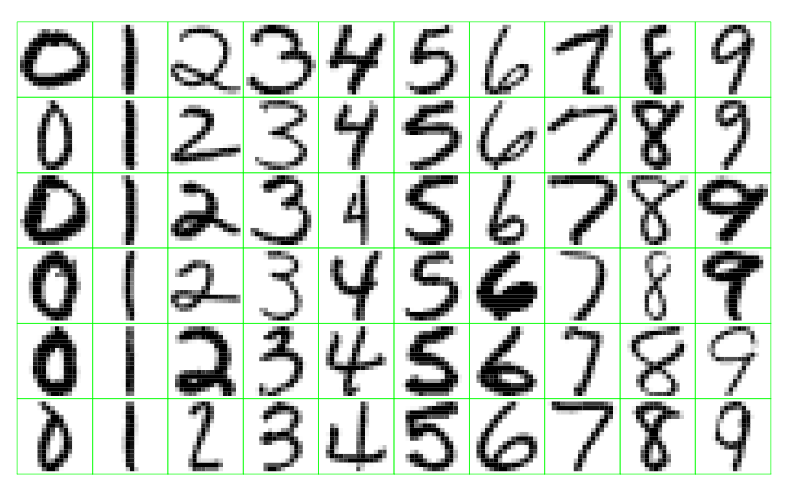
\includegraphics[width=0.7\textwidth,height=\textheight]{digits.png}
\vspace{1mm}

\flushleft

Examples of handwritten digits from U.S. postal envelopes. \scriptsize
Image taken from \url{https://web.stanford.edu/~hastie/ElemStatLearnII/}
\end{block}
\end{frame}

\begin{frame}
\begin{block}{Example 2: Email classification (spam detection)}
\protect\hypertarget{example-2-email-classification-spam-detection}{}
\(~\)

\begin{itemize}
\tightlist
\item
  Goal: to build a spam filter.
\end{itemize}

\vspace{1mm}

\begin{itemize}
\tightlist
\item
  This filter can based on the frequencies of words and characters in
  emails.
\end{itemize}

\(~\)

The table below shows the average percentage of words or characters in
an email message, based on 4601 emails of which 1813 were classified as
a spam.

\begin{longtable}[]{@{}lrrrrrr@{}}
\toprule\noalign{}
& you & free & george & ! & \$ & edu \\
\midrule\noalign{}
\endhead
not spam & 1.27 & 0.07 & 1.27 & 0.11 & 0.01 & 0.29 \\
spam & 2.26 & 0.52 & 0.00 & 0.51 & 0.17 & 0.01 \\
\bottomrule\noalign{}
\end{longtable}
\end{block}
\end{frame}

\begin{frame}{The Supervised Learning Problem}
\protect\hypertarget{the-supervised-learning-problem}{}
\textcolor{blue}{\emph{Starting point}}:

\begin{itemize}
\item
  Outcome measurement \(Y\), also called dependent variable, response,
  target.
\item
  Vector of \(p\) predictor measurements \(X=(X_1,\ldots,X_p)\), also
  called inputs, regressors, covariates, features, independent
  variables.
\item
  In the \textbf{regression problem}, \(Y\) is quantitative (e.g price,
  blood pressure).
\item
  In the \textbf{classification problem}, \(Y\) takes values in a
  finite, unordered set (survived/died, digit 0-9, cancer class of
  tissue sample).
\item
  We have training data \((x_1, y_1), \ldots , (x_N , y_N )\). These are
  observations (examples, instances) of these measurements.
\end{itemize}
\end{frame}

\begin{frame}
\begin{block}{Supervised learning and its objectives}
\protect\hypertarget{supervised-learning-and-its-objectives}{}
\vspace{2mm}

Our data set (training set) consists of \(n\) measurement of the
response variable \(Y\) and of \(p\) covariates \(x\):
\[(y_1, x_{11}, x_{12},\ldots, x_{1p}), (y_2, x_{21},\ldots, x_{2p}), \ldots, (y_n, x_{n1}, x_{n2},\ldots, x_{np}).\]
\(~\)

On the basis of the \emph{training data} we would like to:

\begin{itemize}
\item
  \textbf{accurately predict} unseen test cases.
\item
  \textbf{understand} which input affects the outcomes, and how.
\item
  \textbf{assess the quality} of your predictions and inference.
\end{itemize}

\vspace{2mm}

The majority of problems studied in this course fall in the supervised
learning category (exception: Module 10)
\end{block}
\end{frame}

\begin{frame}{Notation and key statistical concepts}
\protect\hypertarget{notation-and-key-statistical-concepts}{}
See notes and p.~9--12 in the course book.

\vspace{6cm}
\end{frame}

\begin{frame}{The Unsupervised Learning Problem}
\protect\hypertarget{the-unsupervised-learning-problem}{}
\begin{itemize}
\item
  There is \textbf{no outcome variable} \(y\), just a set of predictors
  (features) \(x_i\) measured on a set of samples.
\item
  Objective is more fuzzy -- find (hidden) patterns or groupings in the
  data - in order to \emph{gain insight and understanding}. There is no
  \emph{correct} answer.
\item
  Difficult to know how well your are doing.
\end{itemize}

\(~\)

Examples in the course:

\begin{itemize}
\tightlist
\item
  Clustering (M10)
\item
  Principal component analysis (M10)
\end{itemize}
\end{frame}

\begin{frame}{Overall philosophy}
\protect\hypertarget{overall-philosophy}{}
\begin{itemize}
\tightlist
\item
  Important to understand the simpler methods first, in order to grasp
  the more sophisticated ones.
\end{itemize}

\(\rightarrow\) \textbf{Simpler methods often perform as well as fancier
ones!}

\(~\)

\begin{itemize}
\tightlist
\item
  It is important to accurately \emph{assess the performance of a
  method}, to know how well or how badly it is working.
\end{itemize}
\end{frame}

\begin{frame}{Statistical Learning vs.~Machine Learning}
\protect\hypertarget{statistical-learning-vs.-machine-learning}{}
\begin{itemize}
\item
  Machine learning arose as a subfield of Artificial Intelligence.
\item
  Statistical learning arose as a subfield of Statistics.
\item
  There is much overlap -- both fields focus on supervised and
  unsupervised problems:

  \begin{itemize}
  \tightlist
  \item
    Machine learning has a greater emphasis on large scale applications
    and prediction accuracy.
  \item
    Statistical learning emphasizes models and their interpretability,
    and precision and uncertainty.
  \end{itemize}
\item
  The distinction has become more and more blurred, and there is a great
  deal of ``cross-fertilization''.
\item
  Machine learning has the upper hand in Marketing!
\end{itemize}
\end{frame}

\begin{frame}
\begin{itemize}
\item
  There is a controversy and some scepticism against ``too fancy'\,' ML
  methods.
\item
  Criticism: ML often re-invents existing methods and names them
  differently, but often without awareness of existing methods in
  statistics.
\item
  Almost weekly new literature that delivers comparison. Often, the
  ``simple'' statistical methods ``win''.
\end{itemize}

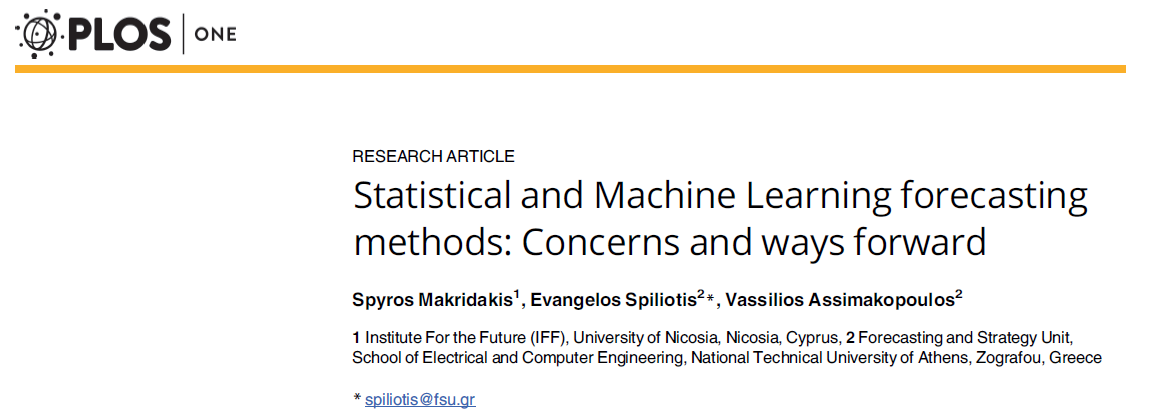
\includegraphics{ML_vs_stat.png}
\end{frame}

\begin{frame}
A tweet by one of the co-authors of the course book,
coincidentially\ldots{}

\%
\includegraphics{AI_ML_stat.png}
\end{frame}

\begin{frame}
\begin{block}{What is the aim in statistical learning?}
\protect\hypertarget{what-is-the-aim-in-statistical-learning}{}
\vspace{3mm}

We are talking about supervised methods now. Assume:

\vspace{2mm}

\begin{itemize}
\tightlist
\item
  we observe one \emph{quantitative} response \(Y\) and \(p\) different
  predictors \(x_1, x_2,... , x_p\).
\end{itemize}

\vspace{1mm}

\begin{itemize}
\tightlist
\item
  We assume that there is a function \(f\) that relates the response and
  the predictor variables: \[ Y = f(x) + \varepsilon,\] where
  \(\varepsilon\) is a random error term with mean 0 and independent of
  \(x\).
\end{itemize}

\(~\)

\centering

\{\bf The aim is to estimate $f$.\}
\end{block}
\end{frame}

\begin{frame}{Example 1}
\protect\hypertarget{example-1}{}
Sales of a product, given advertising budgets in different media.

\includegraphics{../../ISLR/Figures/Chapter2/2.1.pdf}
\end{frame}

\begin{frame}{Example 2}
\protect\hypertarget{example-2}{}
\vspace{4mm}

Income for given levels of education.

\includegraphics{../../ISLR/Figures/Chapter2/2.2.pdf}
\end{frame}

\begin{frame}
There are two main reasons for estimating \(f\):

\begin{itemize}
\item
  \textbf{Prediction}
\item
  \textbf{Inference}
\end{itemize}
\end{frame}

\begin{frame}
\begin{block}{Reason 1: Prediction}
\protect\hypertarget{reason-1-prediction}{}
\(~\)

\textbf{Aim}: predict a response \(Y\) given new observations \(x\) of
the covariates as accurately as possible.

\(~\)

Notation:

\[\hat{Y} = \hat{f}(x).\]

\begin{itemize}
\item
  \(\hat{f}\): estimated \(f\)
\item
  \(\hat{Y}\) prediction for \(Y\) given \(x\).
\end{itemize}

\vspace{2mm}

\begin{itemize}
\tightlist
\item
  We \emph{do not really care} about the shape of \(f\) (``black
  box'').\\
  \(\rightarrow\) no interpretation of regression parameters when the
  aim is purely prediction!
\end{itemize}
\end{block}
\end{frame}

\begin{frame}
There are two quantities which influence the accuracy of \(\hat{Y}\) as
a prediction of \(Y\):

\begin{itemize}
\tightlist
\item
  The \emph{\textcolor{red}{reducible error}} has to do with our
  estimate \(\hat{f}\) of \(f\). This error can be reduced by using the
  most \emph{appropriate} statistical learning technique.
\item
  The \emph{\textcolor{red}{irreducible error}} comes from the error
  term \(\varepsilon\) and cannot be reduced by improving \(f\). This is
  related to the unobserved quantities influencing the response and
  possibly the randomness of the situation.
\end{itemize}

For a \textbf{given} \(\hat{f}\) and a set of predictors \(X\) which
gives \(\hat{Y}=\hat{f}(X)\), we have

\[\text{E}[(Y-\hat{Y})^2] = \underbrace{(f(X)-\hat{f}(X))^2}_{reducible} + \underbrace{\text{Var}(\epsilon)}_{irreducible}\]
\end{frame}

\begin{frame}
\begin{block}{Q: If there were a \emph{deterministic} relationship
between the response and a set of predictors, would there then be both
reducible and irreducible error?}
\protect\hypertarget{q-if-there-were-a-deterministic-relationship-between-the-response-and-a-set-of-predictors-would-there-then-be-both-reducible-and-irreducible-error}{}
\end{block}
\end{frame}

\begin{frame}
\begin{block}{Reason 2: Inference}
\protect\hypertarget{reason-2-inference}{}
\(~\)

\textbf{Aim}: understand \emph{how} the response variable is affected by
the various predictors (covariates).

\(~\)

The \emph{exact form} of \(\hat{f}\) is of \emph{main interest}.

\vspace{2mm}

\begin{itemize}
\tightlist
\item
  Which predictors are associated with the response?
\item
  What is the relationship between the response and each predictor?
\item
  Can the relationship be linear, or is a more complex model needed?
\end{itemize}
\end{block}
\end{frame}

\begin{frame}{Estimating \(f\)}
\protect\hypertarget{estimating-f}{}
Overall idea:

\begin{itemize}
\tightlist
\item
  Using available \emph{training data} \((x_1,y_n),\ldots (x_n,y_n)\) to
  estimate \(\hat{f}\), such that \(Y\approx \hat{f}(X)\) for any
  \((X,Y)\) (also those that have not yet been observed).
\end{itemize}

\(~\)

\textcolor{red}{Two main approaches:}

\begin{itemize}
\tightlist
\item
  Parametric methods
\item
  Non-parametric methods
\end{itemize}
\end{frame}

\begin{frame}
\begin{block}{Parametric methods}
\protect\hypertarget{parametric-methods}{}
\(~\)

Assumption about the form or shape of the function \(f\).

The multiple linear model (M3) is an example of a parametric method:

\[f(x) = \beta_0 + \beta_1 x_1 + ... + \beta_p x_p+\varepsilon \ , \]

with \(\varepsilon \sim N(0,\sigma^2)\).

\(~\)

The task simplifies to finding estimates of the \(p+1\) coefficients
\(\beta_0, \beta_1, .. ,\beta_p\). To do this we use the training data
to fit the model, such that
\[Y \approx \hat{\beta_0} + \hat{\beta_1} x_1 + ... + \hat{\beta_p} x_p \ .\]
\end{block}
\end{frame}

\begin{frame}
Fitting a parametric models is thus done in two steps:

\begin{enumerate}
\tightlist
\item
  Select a form for the function \(f\).\\
\item
  Estimate the unknown parameters in \(f\) using the training set.
\end{enumerate}
\end{frame}

\begin{frame}
\begin{block}{Non-parametric methods}
\protect\hypertarget{non-parametric-methods}{}
\(~\)

\begin{itemize}
\tightlist
\item
  Non-parametric methods seek an estimate of \(f\) that gets close to
  the data points, but without making explicit assumptions about the
  form of the function \(f\).
\end{itemize}

\vspace{2mm}

\begin{itemize}
\tightlist
\item
  Example: \(K\)-nearest neighbour (KNN) algorithm, used in
  classification. KNN predicts a class membership for a new observation
  by making a majority vote based on its \(K\) nearest neighbours. We
  will discuss the \(K\)-nearest neighbour algorithm in Module 4.
\end{itemize}
\end{block}
\end{frame}

\begin{frame}
\begin{block}{KNN example}
\protect\hypertarget{knn-example}{}
\(~\)

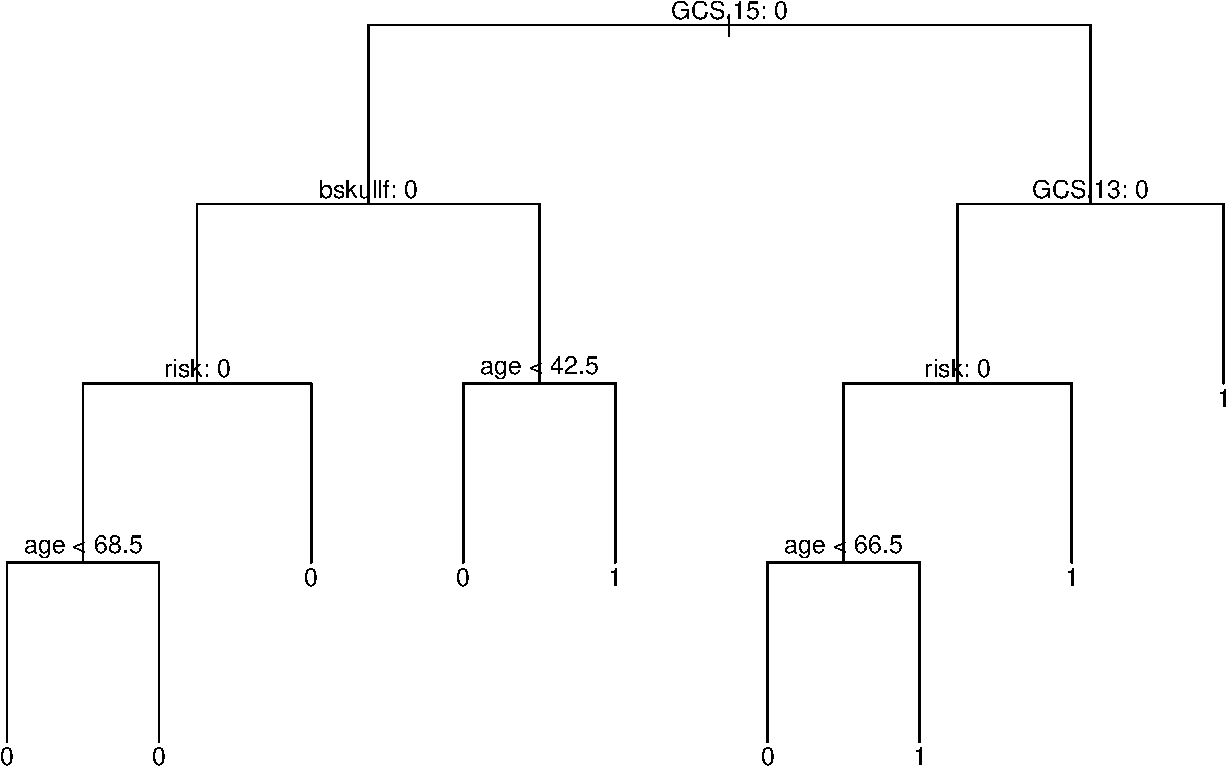
\includegraphics{2StatLearn.1_files/figure-beamer/unnamed-chunk-2-1.pdf}
\end{block}
\end{frame}

\begin{frame}
\begin{block}{Parametric methods}
\protect\hypertarget{parametric-methods-1}{}
\begin{longtable}[]{@{}
  >{\raggedright\arraybackslash}p{(\columnwidth - 2\tabcolsep) * \real{0.5000}}
  >{\raggedright\arraybackslash}p{(\columnwidth - 2\tabcolsep) * \real{0.5000}}@{}}
\toprule\noalign{}
\begin{minipage}[b]{\linewidth}\raggedright
Advantages
\end{minipage} & \begin{minipage}[b]{\linewidth}\raggedright
Disadvantages
\end{minipage} \\
\midrule\noalign{}
\endhead
Simple to use and easy to understand & The function \(f\) is constrained
to the specified form.\vspace{2mm} \\
Requires little training data & The assumed function form of \(f\) will
in general not match the true function, potentially giving a poor
estimate.\vspace{2mm} \\
Computationally cheap & Limited flexibility \\
\bottomrule\noalign{}
\end{longtable}
\end{block}
\end{frame}

\begin{frame}
\begin{block}{Non-parametric methods}
\protect\hypertarget{non-parametric-methods-1}{}
\begin{longtable}[]{@{}
  >{\raggedright\arraybackslash}p{(\columnwidth - 2\tabcolsep) * \real{0.5000}}
  >{\raggedright\arraybackslash}p{(\columnwidth - 2\tabcolsep) * \real{0.5000}}@{}}
\toprule\noalign{}
\begin{minipage}[b]{\linewidth}\raggedright
Advantages
\end{minipage} & \begin{minipage}[b]{\linewidth}\raggedright
Disadvantages
\end{minipage} \\
\midrule\noalign{}
\endhead
Flexible: a large number of functional forms can be fitted & Can overfit
the data\vspace{6mm} \\
No strong assumptions about the underlying function are made &
Computationally more expensive as more parameters need to be
estimated\vspace{3mm} \\
Can often give good predictions & Much data are required to estimate
(the complex) \(f\). \\
\bottomrule\noalign{}
\end{longtable}
\end{block}
\end{frame}

\begin{frame}{Prediction accuracy vs.~interpretability}
\protect\hypertarget{prediction-accuracy-vs.-interpretability}{}
(we are warming up to the bias--variance trade--off)

\textbf{Inflexible} methods:

\begin{itemize}
\tightlist
\item
  Linear regression (M3)
\item
  Linear discriminant analysis (M4)
\item
  Subset selection and lasso (M6)
\end{itemize}

\textbf{Flexible} methods:

\begin{itemize}
\tightlist
\item
  KNN classification (M4), KNN regression, Smoothing splines (M7)
\item
  Bagging and boosting (M8 adn M9)
\item
  Neural networks (M11)
\end{itemize}
\end{frame}

\begin{frame}
\begin{block}{Why would I ever prefer an inflexible method?}
\protect\hypertarget{why-would-i-ever-prefer-an-inflexible-method}{}
\(~\)

Example: Prediction of icome from ``Years of Education'' and
``Seniority''\vspace{2mm}

\centering

\includegraphics[width=0.43\textwidth,height=\textheight]{../../ISLR/Figures/Chapter2/2.4.pdf}

\includegraphics[width=0.45\textwidth,height=\textheight]{../../ISLR/Figures/Chapter2/2.6.pdf}

A linear model vs a perfect fit.
\end{block}
\end{frame}

\begin{frame}
\(~\)

\textbf{Potential problems:}

\textbf{Overfitting} occurs when the estimated function \(f\) is too
closely fit to the observed data points.

\textbf{Underfitting} occurs when the estimated function \(f\) is too
rigid to capture the underlying structure of the data.

\(~\)

\emph{We illustrate this by a toy example using polynomial regression.}
\end{frame}

\begin{frame}
\begin{block}{Polynomial regression example (simulation)}
\protect\hypertarget{polynomial-regression-example-simulation}{}
Consider a covariate \(x\) observed between \(x=-2, \ldots , 4\) and
\(n=61\) observations.

\begin{center}\includegraphics{2StatLearn.1_files/figure-beamer/data-1} \end{center}
\end{block}
\end{frame}

\begin{frame}
We know that the true data generating model consist in a quadratic
relationship between response \(Y\) and covariate \(x\)

\[ Y=x^2 + \epsilon\]

with error (noise) term \(\varepsilon\sim N(0,\sigma^2)\) with
\(\sigma=2\). It is a substitue for all the unobserved variables that
are not in our equation, but that might influence \(Y\).

\begin{itemize}
\tightlist
\item
  We call \(Y=x^2\) the \emph{truth}.
\item
  \(\varepsilon\) is the \emph{irreducible error}.
\end{itemize}
\end{frame}

\begin{frame}
\begin{center}\includegraphics{2StatLearn.1_files/figure-beamer/truth-1} \end{center}
\end{frame}

\begin{frame}
Try to fit a function to the observations \emph{assuming we do not know}
the true relationship:

\(~\)

\begin{itemize}
\tightlist
\item
  \textbf{poly1}: Simple linear model of the form \(\beta_0+\beta_1 x\)
  fitted to the observations.
\end{itemize}

\begin{itemize}
\tightlist
\item
  \textbf{poly2}: Quadratic polynomial fit to the data, of the form
  \(\beta_0+\beta_1 x +\beta_2 x^2\).
\end{itemize}

\begin{itemize}
\tightlist
\item
  \textbf{poly10}: Polynomial of degree 10 fit of the form
  \(\beta_0+\beta_1 x +\beta_2 x^2+\cdots +\beta_{10}x^{10}\)
\end{itemize}

\begin{itemize}
\tightlist
\item
  \textbf{poly20}: Polynomial of degree 10 fit of the form
  \(\beta_0+\beta_1 x +\beta_2 x^2+\cdots +\beta_{20}x^{20}\)
\end{itemize}
\end{frame}

\begin{frame}
\begin{center}\includegraphics{2StatLearn.1_files/figure-beamer/overunderfit-1} \end{center}

The degree of the polynomial is a \emph{flexibility parameter}.
\end{frame}

\begin{frame}
We can now ask:

\begin{itemize}
\item
  Which of these models performs ``best''?
\item
  Is there \emph{one} method that dominates all others?
\end{itemize}
\end{frame}

\begin{frame}{Assessing model accuracy}
\protect\hypertarget{assessing-model-accuracy}{}
\textbf{No method} dominates all others over all possible data sets.

\begin{itemize}
\tightlist
\item
  That is why we need to learn about many different methods.
\item
  For a given data set we need to know how to decide which method
  produces the \emph{best} results.
\item
  We need to understand what \emph{best} means.
\item
  How close is the predicted response to the true response value?
\end{itemize}
\end{frame}

\begin{frame}
\begin{block}{Measuring the Quality of Fit}
\protect\hypertarget{measuring-the-quality-of-fit}{}
\vspace{2mm}

The quality of fit can be measures as the \emph{Training MSE} (mean
squared error), using the data that were used to estimate \(f\):

\[ \text{MSE}_{\text{train}}=\frac{1}{n}\sum_{i=1}^n (y_i-\hat{f}(x_i))^2\]
\(~\)
\end{block}
\end{frame}

\begin{frame}
\begin{block}{What is the training MSE?}
\protect\hypertarget{what-is-the-training-mse}{}
\begin{center}\includegraphics{2StatLearn.1_files/figure-beamer/unnamed-chunk-3-1} \end{center}
\end{block}
\end{frame}

\begin{frame}
Why is the training MSE not the real measure of interest?

\(~\)

\pause

Examples:

\begin{itemize}
\item
  We don't want to predict last weeks stock price, we want to predict
  the stock price next week.
\item
  We don't want to predict if a patient in the training data has
  diabetes (because we already know this), we want to predict if a new
  patient has diabetes.
\end{itemize}
\end{frame}

\begin{frame}
\begin{block}{Training error for the polynomial example}
\protect\hypertarget{training-error-for-the-polynomial-example}{}
\(~\)

\begin{center}\includegraphics[width=0.8\linewidth]{2StatLearn.1_files/figure-beamer/trainMSE-1} \end{center}

\vspace{2mm}

Left: one repetition, right: 100 repetitions of the training set.

\vspace{2mm}

\textbf{Q}: Based on the training MSE - which model fits the data the
best?
\end{block}
\end{frame}

\begin{frame}
\begin{block}{Test MSE}
\protect\hypertarget{test-mse}{}
\(~\)

\begin{itemize}
\tightlist
\item
  Simple solution: estimate \(\hat{f}\) using the training data (maybe
  my minimizing the training MSE), but choose the \emph{best} model
  using a separate \emph{test set}.
\end{itemize}

\vspace{2mm}

\begin{itemize}
\tightlist
\item
  \emph{Test MSE} for a set of \(n_0\) test observations
  \((x_{0j},y_{0j})\):
\end{itemize}

\[ \text{MSE}_{\text{test}}=\frac{1}{n_0}\sum_{j=1}^{n_0} (y_{0j}-\hat{f}(x_{0j}))^2\]

\vspace{2mm}

\begin{itemize}
\tightlist
\item
  Alternative notation: \[\text{Ave}(y_0-\hat{f}(x_0))^2\] (taking the
  average over all available test observations).
\end{itemize}
\end{block}
\end{frame}

\begin{frame}
\begin{block}{What is the test MSE?}
\protect\hypertarget{what-is-the-test-mse}{}
\begin{center}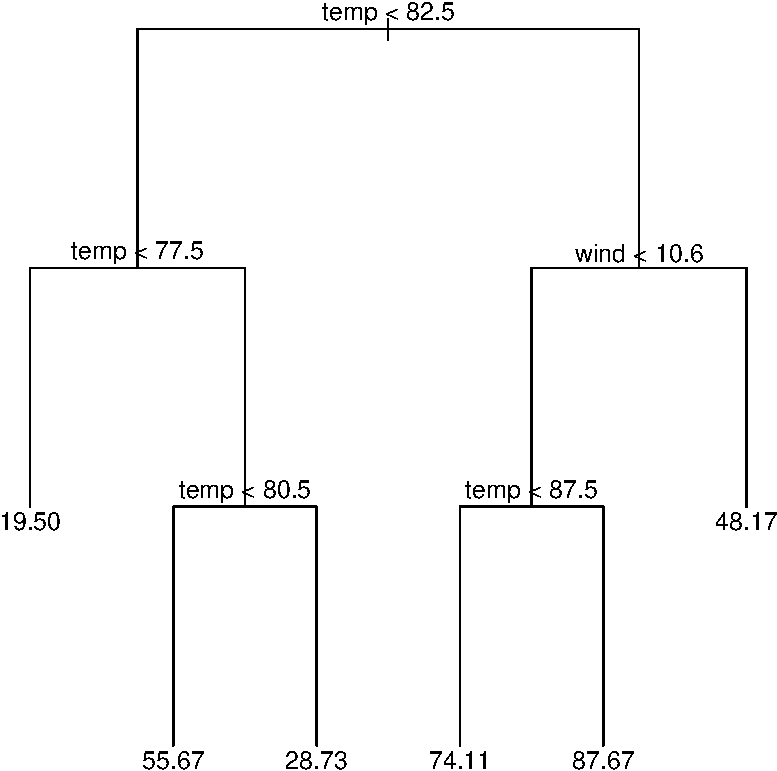
\includegraphics{2StatLearn.1_files/figure-beamer/unnamed-chunk-4-1} \end{center}
\end{block}
\end{frame}

\begin{frame}
\begin{block}{Test error for the polynomial example}
\protect\hypertarget{test-error-for-the-polynomial-example}{}
\(~\)

\begin{center}\includegraphics[width=0.9\linewidth]{2StatLearn.1_files/figure-beamer/traintestMSE-1} \end{center}

Left: one repetition, right: 100 repetitions for the testMSE.
\end{block}
\end{frame}

\begin{frame}
\begin{block}{Questions:}
\protect\hypertarget{questions}{}
\(~\)

\textbf{Q1}: Based on the test MSE - which model fits the data the best?

\vspace{2mm}

\textbf{Q2:} What if we do not have access to test data?

\vspace{2mm}

\textbf{Q3:} Can we instead just use the training data MSE to choose a
model? A low training error should also give a low test error?

\vspace{2mm}

\textbf{Q4:} Important observation:

\vspace{2mm}

\begin{itemize}
\item
  The test error seems to have a minimum (U-shape) in between the
  extremes.
\item
  The training error keeps going down.
\end{itemize}

\centering
\vspace{2mm}

Why?
\end{block}
\end{frame}

\begin{frame}{The Bias-Variance trade-off}
\protect\hypertarget{the-bias-variance-trade-off}{}
\vspace{2mm}

The U-shape is the result of \emph{two competing properties} of
statistical learning methods.

\vspace{2mm}

\begin{itemize}
\tightlist
\item
  Assume we have fitted a \emph{regression} curve
  \[Y  = f(x) + \varepsilon\] to our training data \(\{x_i, y_i\}\) for
  \(i=1,..,n\), and \(\varepsilon\) is an unobserved random variable
  that adds random, uncorrelated, mean-zero noise term with variance
  \(\sigma^2\).\footnote{$\varepsilon$ is a substitute for all the unobserved variables that influence $Y$.}
\end{itemize}

\vspace{2mm}

\begin{itemize}
\tightlist
\item
  The training data was used to estimate \(\hat{f}\).
\end{itemize}
\end{frame}

\begin{frame}
\begin{itemize}
\tightlist
\item
  The \emph{\textcolor{red}{expected test mean squared error (MSE)} at
  \(x_0\)} (unseen test observation) is defined as:
  \[\text{E}[(y_0 - \hat{f}(x_0))^2] \ .\]\\
  This is the average test MSE that we would obtain if we repeatedly
  estimated \(f\) on different training sets.
\end{itemize}

\(~\)

\begin{itemize}
\tightlist
\item
  Compare this to the test MSE for the polynomical example
  (\(\text{MSE}_{\text{test}}\)): The average is simply replaced by the
  \emph{theoretical version} (expected value).
\end{itemize}
\end{frame}

\begin{frame}
Using that \(y_0=f(x_0)+\varepsilon\), this expected test MSE (at
\(X=x_0\)) can be decomposed into three terms (board) \begin{align*}
&\text{E}[(y_0 - \hat{f}(x_0))^2] = \\
& ... \\
& =  \underbrace{\text{Var}(\varepsilon)}_{\text{Irreducible error}} + \underbrace{\text{Var}(\hat{f}(x_0))}_{\text{Variance of prediction}} + \underbrace{\left( f(x_0) - \text{E}[\hat{f}(x_0)] \right)^2}_{\text{Squared bias}}
\end{align*}
\end{frame}

\begin{frame}
\[\text{E}[(y_0 - \hat{f}(x_0))^2]=\cdots=\text{Var}(\varepsilon) +  \text{Var}(\hat{f}(x_0))+[\text{Bias}(\hat{f}(x_0))]^2\]

\begin{itemize}
\item
  \emph{\textcolor{red}{Irreducible error}}. This term cannot be reduced
  regardless how well our statistical model fits the data.
\item
  \emph{\textcolor{red}{Variance}} of the prediction at
  \(\hat{f}(x_0)\). Relates to the amount by which \(\hat{f}(x_0)\) is
  expected to change for different training data. If the variance is
  high, there is large uncertainty associated with the prediction.
\item
  \emph{\textcolor{red}{Squared bias}}. The bias gives an estimate of
  how much the prediction differs from the true mean. If the bias is low
  the model gives a prediction which is close to the true value.
\end{itemize}
\end{frame}

\begin{frame}
\begin{itemize}
\item
  Note: \[\text{E}[(y_0 - \hat{f}(x_0))^2]\] is the \textbf{expected
  test MSE}. We can think of this as the average test MSE we would
  obtain if we repeatedly estimated \(f\) using many training sets (as
  we did in our example), and then tested this estimate at \(x_0\).
\item
  However, if we also assume that \(X\) is a random variable, this is
  actually \(\text{E}[(Y - \hat{f}(x_0))^2 \mid X=x_0]\)
\item
  The \textbf{overall expected test MSE} can be computed by averaging
  the expected test MSE over all possible values of \(x_0\) (averaging
  with respect to frequency in test set).
\item
  Mathematically: \(\text{E} \{ \text{E}[(Y - \hat{f}(X))^2 \mid X]\}\)
  (by the law of total expectation / law of double expectations).
\end{itemize}
\end{frame}

\begin{frame}
\begin{block}{General rule}
\protect\hypertarget{general-rule}{}
\vspace{4mm}

For more flexible models, the variance will \emph{increase} and the bias
will \emph{decrease}.

\vspace{4mm}

\centering

This is called the \emph{\textcolor{red}{Bias-variance trade-off}}.
\end{block}
\end{frame}

\begin{frame}
\begin{block}{Choosing the best model}
\protect\hypertarget{choosing-the-best-model}{}
\(~\)

The aim is often to obtain \textbf{the most predictive model}.
Ingredients:

\vspace{2mm}

\begin{enumerate}
\tightlist
\item
  \textbf{Training set}: The observations used to fit the statistical
  model \(\rightarrow\) Training error
\end{enumerate}

\vspace{2mm}

\begin{enumerate}
\setcounter{enumi}{1}
\tightlist
\item
  \textbf{Test sample}: new observations which were not used when
  fitting the model \(\rightarrow\) Test error
\end{enumerate}

\vspace{4mm}

We have seen that

\vspace{4mm}

\begin{itemize}
\tightlist
\item
  Training error decreases for more complex/flexible models, but the
  test error has an \textbf{optimum}.
\end{itemize}

\centering

\(\rightarrow\) \textbf{Bias-Variance trade-off}
\end{block}
\end{frame}

\begin{frame}
\includegraphics{../../ISLR/Figures/Chapter2/2.12.pdf}

\begin{itemize}
\tightlist
\item
  Inflexible models: may lead to a poor fit (high bias).
\item
  Flexible (complex) models: may overfit the data (high variance).
\item
  Aim: find the optimum where the
  \emph{\textcolor{red}{test MSE is minimal}}.
\end{itemize}
\end{frame}

\begin{frame}
\begin{block}{Polynomial example (cont.)}
\protect\hypertarget{polynomial-example-cont.}{}
See recommended exercise 2.

\vspace{2mm}

\(Y=x^2\) is still the \emph{truth}.

\vspace{2mm}

\begin{center}\includegraphics[width=0.9\linewidth]{2StatLearn.1_files/figure-beamer/biasvarianceforx-1} \end{center}

For four different polynomial models (poly1,2,10 and 20), the squared
bias, variance, irreducible error and the total sum. Plots based on 100
simulations for the polynomial example.
\end{block}
\end{frame}

\begin{frame}
\begin{center}\includegraphics{2StatLearn.1_files/figure-beamer/biasvarianceforpoly-1} \end{center}

At four different values for \(x_0\), the squared bias, variance,
irreducible error and the total sum. Plots based on 100 simulations for
the polynomial example.
\end{frame}

\begin{frame}
\begin{center}\includegraphics[width=0.9\linewidth]{2StatLearn.1_files/figure-beamer/averageoverxs-1} \end{center}

Overall version (averaging over 61 gridpoints of \(x\)).
\end{frame}

\begin{frame}{Main Concepts}
\protect\hypertarget{main-concepts}{}
\begin{itemize}
\tightlist
\item
  Prediction and Inference
\item
  Reducible and Irreducible Error
\item
  Training and Test Set
\item
  Bias-Variance Trade off
\end{itemize}
\end{frame}

\begin{frame}
\end{frame}

\end{document}
